\chapter{Результаты обучения физически-информированной нейронной сети}
Проводилось обучение сети на задаче "течение Куэтта" с использованием функций активации REAct.
В результате первого этапа обучения модель с предсказанным минимальным отклонением от
верного решения (рис. \ref{fig:couette_react_best}) имела следующие значения
гиперпараметров (табл. \ref{table:couette_react_best_params}).

\begin{table}[ht]
    \centering
    \caption{Значения гиперпараметров у модели с лучшим результатом}
    \begin{tabular}{ |c|c| } 
        \hline
        Функция активации & $\text{REAct}(0.8, -4, -3.2, 0.2)$ \\
        \hline
        Оптимизатор & Adagrad \\ 
        \hline
        Конфигурация сети & $64-16-32$ \\ 
        \hline
        Скорость обучения & $10^{-3}$ \\ 
        \hline
        Количество точек внутри области & $100$ \\ 
        \hline
    \end{tabular}
    \label{table:couette_react_best_params}
\end{table}

В результате анализа остальных моделей было подсчитано количество нулевых
решений, решений с максимальным отклонением до 20\%, а также больше 20\% и 50\%.
Помимо перечисленных также было несколько моделей, ушедших в процессе обучения в
NaN (рис. \ref{fig:couette_react_stat}).

\begin{figure}[ht]
    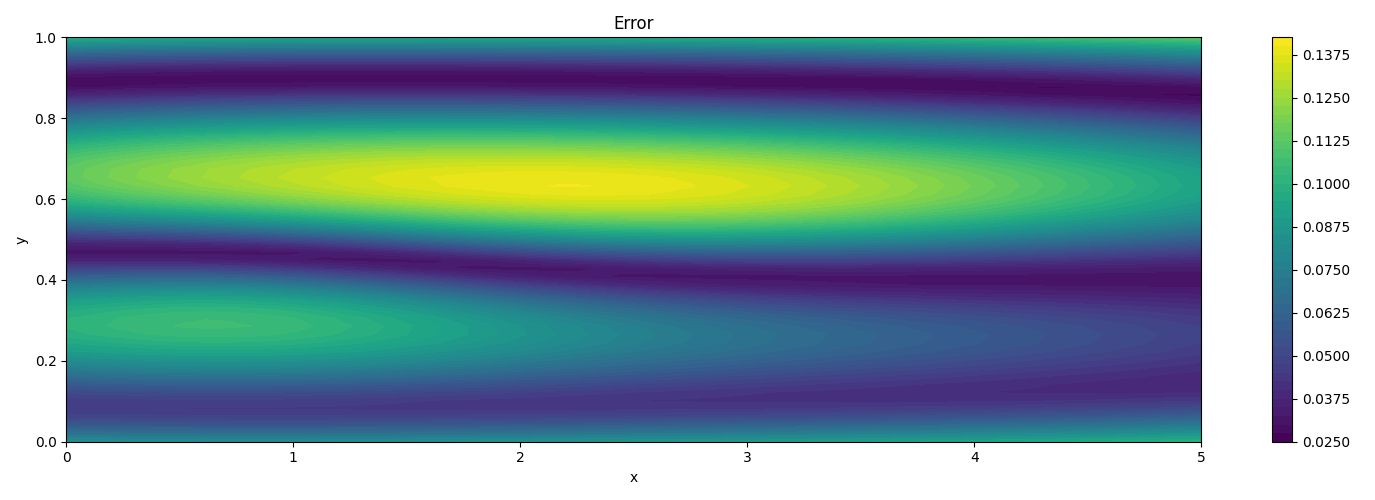
\includegraphics{data/couette_react_error_best.png}
    \caption{Результат с минимальным показателем отклонения от точного решения в процессе обучения и
    кроссвалидации модели с функцией активации REAct}
    \label{fig:couette_react_best}
\end{figure}
Также стоит отметить, что все нулевые решения соответствовали функции активации,
которая на всей области определения имеет отрицательные значения.

\begin{figure}[ht]
    \centering
    \begin{tikzpicture}
        \pgfplotstableread{
        Label   First
        NaN                     4
        Нулевое\ решение        30
        $>50\%$                 16
        $>20\%$                 94
        $<20\%$                 17
        }\datatable
        
        \begin{axis}[
            xbar stacked,
            xmin=0,
            ytick=data,
            yticklabels from table={\datatable}{Label}
            ]
            \addplot [fill=yellow] table [x=First, y expr=\coordindex] {\datatable};
        \end{axis}
    \end{tikzpicture}
    \caption{Распределение результатов кроссвалидации с функцией активации REAct}
    \label{fig:couette_react_stat}
\end{figure}

В качестве корректных параметров были отобраны те, которые соответствуют критерию
принадлежности к группе с уровнем менее 20\%. В результате, во второй этап были
включены следующие параметры:
\begin{enumerate}
    \item Конфигурации с резким переходом между слоями ($16-64-32$ и $64-16-32$) а также
    с линейным переходом ($16-32-64$ и $64-32-16$) не показали особых результатов по
    сравнению с остальными трехслойными сетями. Аналогично конфигурации
    $16-16$ и $32-32$ показали себя хуже по сравнению с $64-64$.
    \item По количеству точек внутри области значительно больше удачных
    результатов было при $100$ точек. Это поведение характеризуется 
    соотношением точек на границе и внутри области. Данное соотношение 
    показывает значимость граничных условий, что необходимо для избегания
    нулевого решения
    \item Скорость обучения влияет на то, сможет ли оптимизатор 
    выбраться из локального минимума. Лучший результат показало значение
    скорости обучения равное $10^{-3}$
    \item Среди оптимизаторов лучшие результаты показали \textbf{Adam}, \textbf{Adagrad} и
    \textbf{ASGD}, в свою очередь \textbf{Adamax} и \textbf{RSMProp} являются узкоспециализированными,
    что требует точной настройки параметров, что в данной работе не рассматривается.
\end{enumerate} 

Теперь получив более точное представление о наших параметрах можно приступить
ко второму этапу.

В представленных ниже графиках показано сравнение результатов работы нейронной сети
при различных гиперпараметрах. Такой подход позволяет детально проанализировать
влияние каждого параметра на общую эффективность модели и выявить, какие параметры
обеспечивают наилучшее качество обучения.
\begin{figure}[ht]
    \centering
    \begin{subfigure}[b]{0.4\textwidth}
        \begin{tikzpicture}
            \begin{axis}[
                ymode=log,
                % xlabel={Эпоха},
                ylabel={Медиана},
                xmin=0,
                xtick distance=4000,
                axis lines=left,
                grid=both,
                title={Нижняя граница},
                width=\textwidth
            ]
            \addplot+[mark=*, mark size=1pt, thick, red] table[x=step, y=value, col sep=comma]{data/couette_abu/loss/bc_bottom_neurons_(32, 64, 32).csv};
            \addplot+[mark=*, mark size=1pt, thick, green] table[x=step, y=value, col sep=comma]{data/couette_abu/loss/bc_bottom_neurons_(64, 32, 64).csv};
            \addplot+[mark=*, mark size=1pt, thick, blue] table[x=step, y=value, col sep=comma]{data/couette_abu/loss/bc_bottom_neurons_(64, 64).csv};
            \addplot+[mark=*, mark size=1pt, thick, orange] table[x=step, y=value, col sep=comma]{data/couette_abu/loss/bc_bottom_neurons_(128, 128).csv};
            \end{axis}
        \end{tikzpicture}
        \label{fig:bc_bottom}
    \end{subfigure}
    \hspace{0.5cm}
    \begin{subfigure}[b]{0.4\textwidth}
        \begin{tikzpicture}
            \begin{axis}[
                ymode=log,
                % xlabel={Эпоха},
                % ylabel={Медиана},
                xmin=0,
                xtick distance=4000,
                axis lines=left,
                grid=both,
                title={Верхняя граница},
                width=\textwidth
            ]
            \addplot+[mark=*, mark size=1pt, thick, red] table[x=step, y=value, col sep=comma]{data/couette_abu/loss/bc_top_neurons_(32, 64, 32).csv};
            \addplot+[mark=*, mark size=1pt, thick, green] table[x=step, y=value, col sep=comma]{data/couette_abu/loss/bc_top_neurons_(64, 32, 64).csv};
            \addplot+[mark=*, mark size=1pt, thick, blue] table[x=step, y=value, col sep=comma]{data/couette_abu/loss/bc_top_neurons_(64, 64).csv};
            \addplot+[mark=*, mark size=1pt, thick, orange] table[x=step, y=value, col sep=comma]{data/couette_abu/loss/bc_top_neurons_(128, 128).csv};
            \end{axis}
        \end{tikzpicture}
        \label{fig:bc_top}
    \end{subfigure}
    \vspace{0.05cm}
    \begin{subfigure}[b]{0.4\textwidth}
        \begin{tikzpicture}
            \begin{axis}[
                ymode=log,
                xlabel={Эпоха},
                ylabel={Медиана},
                xmin=0,
                xtick distance=4000,
                axis lines=left,
                grid=both,
                title={Левая граница},
                width=\textwidth
            ]
            \addplot+[mark=*, mark size=1pt, thick, red] table[x=step, y=value, col sep=comma]{data/couette_abu/loss/bc_left_neurons_(32, 64, 32).csv};
            \addplot+[mark=*, mark size=1pt, thick, green] table[x=step, y=value, col sep=comma]{data/couette_abu/loss/bc_left_neurons_(64, 32, 64).csv};
            \addplot+[mark=*, mark size=1pt, thick, blue] table[x=step, y=value, col sep=comma]{data/couette_abu/loss/bc_left_neurons_(64, 64).csv};
            \addplot+[mark=*, mark size=1pt, thick, orange] table[x=step, y=value, col sep=comma]{data/couette_abu/loss/bc_left_neurons_(128, 128).csv};
            \end{axis}
        \end{tikzpicture}
        \label{fig:bc_left}
    \end{subfigure}
    \hspace{0.5cm}
    \begin{subfigure}[b]{0.4\textwidth}
        \begin{tikzpicture}
            \begin{axis}[
                ymode=log,
                xlabel={Эпоха},
                % ylabel={Медиана},
                xmin=0,
                xtick distance=4000,
                axis lines=left,
                grid=both,
                title={Правая граница},
                width=\textwidth
            ]
            \addplot+[mark=*, mark size=1pt, thick, red] table[x=step, y=value, col sep=comma]{data/couette_abu/loss/bc_right_neurons_(32, 64, 32).csv};
            \addplot+[mark=*, mark size=1pt, thick, green] table[x=step, y=value, col sep=comma]{data/couette_abu/loss/bc_right_neurons_(64, 32, 64).csv};
            \addplot+[mark=*, mark size=1pt, thick, blue] table[x=step, y=value, col sep=comma]{data/couette_abu/loss/bc_right_neurons_(64, 64).csv};
            \addplot+[mark=*, mark size=1pt, thick, orange] table[x=step, y=value, col sep=comma]{data/couette_abu/loss/bc_right_neurons_(128, 128).csv};
            \end{axis}
        \end{tikzpicture}
        \label{fig:bc_right}
    \end{subfigure}
    \caption{Зависимость медианы функции потерь на каждой эпохе при разной конфигурации нейронной сети}
    \label{fig:bc_loss_neurons}
\end{figure}

%%%%%%%%%%%%%%%%%%%%%%%%%%%%%%%%%%%%%%%%%%%%%%%%%%%%%%%%%%%%%%%%%%%%%%%%%%%%%%

\begin{figure}[htbp]
    \centering
    \begin{subfigure}[b]{0.4\textwidth}
        \begin{tikzpicture}
            \begin{axis}[
                ymode=log,
                ymin=1e-4, ymax=1e-2,
                xlabel={Эпоха},
                ylabel={Медиана},
                xmin=0,
                xtick distance=4000,
                axis lines=left,
                grid=both,
                title={Уравнение для $v_x$},
                width=\textwidth
            ]
            \addplot+[mark=*, mark size=1pt, thick, red] table[x=step, y=value, col sep=comma]{data/couette_abu/loss/pde_momentum_x_neurons_(32, 64, 32).csv};
            \addplot+[mark=*, mark size=1pt, thick, green] table[x=step, y=value, col sep=comma]{data/couette_abu/loss/pde_momentum_x_neurons_(64, 32, 64).csv};
            \addplot+[mark=*, mark size=1pt, thick, blue] table[x=step, y=value, col sep=comma]{data/couette_abu/loss/pde_momentum_x_neurons_(64, 64).csv};
            \addplot+[mark=*, mark size=1pt, thick, orange] table[x=step, y=value, col sep=comma]{data/couette_abu/loss/pde_momentum_x_neurons_(128, 128).csv};
            \end{axis}
        \end{tikzpicture}
    \end{subfigure}
    \hspace{0.5cm}
    \begin{subfigure}[b]{0.4\textwidth}
        \begin{tikzpicture}
            \begin{axis}[
                ymode=log,
                ymin=1e-4, ymax=1e-2,
                xlabel={Эпоха},
                % ylabel={Медиана},
                xmin=0,
                xtick distance=4000,
                axis lines=left,
                grid=both,
                title={Уравнение для $v_y$},
                width=\textwidth
            ]
            \addplot+[mark=*, mark size=1pt, thick, red] table[x=step, y=value, col sep=comma]{data/couette_abu/loss/pde_momentum_y_neurons_(32, 64, 32).csv};
            \addplot+[mark=*, mark size=1pt, thick, green] table[x=step, y=value, col sep=comma]{data/couette_abu/loss/pde_momentum_y_neurons_(64, 32, 64).csv};
            \addplot+[mark=*, mark size=1pt, thick, blue] table[x=step, y=value, col sep=comma]{data/couette_abu/loss/pde_momentum_y_neurons_(64, 64).csv};
            \addplot+[mark=*, mark size=1pt, thick, orange] table[x=step, y=value, col sep=comma]{data/couette_abu/loss/pde_momentum_y_neurons_(128, 128).csv};
            \end{axis}
        \end{tikzpicture}
    \end{subfigure}
    \begin{subfigure}[b]{0.7\textwidth}
        \begin{tikzpicture}
            \begin{axis}[
                ymode=log,
                ymin=1e-4, ymax=1e-2,
                xlabel={Эпоха},
                ylabel={Медиана},
                xmin=0,
                xtick distance=1000,
                axis lines=left,
                grid=both,
                title={Уравнение непрерывности},
                width=\textwidth
            ]
            \addplot+[mark=*, mark size=1pt, thick, red] table[x=step, y=value, col sep=comma]{data/couette_abu/loss/pde_continuity_neurons_(32, 64, 32).csv};
            % \addlegendentry{(32, 64, 32)}
            \addplot+[mark=*, mark size=1pt, thick, green] table[x=step, y=value, col sep=comma]{data/couette_abu/loss/pde_continuity_neurons_(64, 32, 64).csv};
            % \addlegendentry{(64, 32, 64)}
            \addplot+[mark=*, mark size=1pt, thick, blue] table[x=step, y=value, col sep=comma]{data/couette_abu/loss/pde_continuity_neurons_(64, 64).csv};
            % \addlegendentry{(64, 64)}
            \addplot+[mark=*, mark size=1pt, thick, orange] table[x=step, y=value, col sep=comma]{data/couette_abu/loss/pde_continuity_neurons_(128, 128).csv};
            % \addlegendentry{(128, 128)}
        \end{axis}
        \end{tikzpicture}
    \end{subfigure}
    \caption{Функция потерь для уравнений Навье-Стокса \eqref{eq:navier_stockes} при разной конфигурации нейронной сети}
    \label{fig:pde_loss_neurons}
\end{figure}

%%%%%%%%%%%%%%%%%%%%%%%%%%%%%%%%%%%%%%%%%%%%%%%%%%%%%%%%%%%%%%%%%%

\begin{figure}[htbp]
    \centering
    \begin{tikzpicture}
        \begin{axis}[
            width=0.8\textwidth,
            ymode=log,
            xlabel={Эпоха},
            ylabel={Медиана},
            xmin=0,
            xtick distance=1000,
            axis lines=left,
            grid=both,
        ]
            \addplot+[mark=*, mark size=1pt, thick, red] table[x=step, y=value, col sep=comma]{data/couette_abu/loss/total_loss_neurons_(32, 64, 32).csv};
            \addlegendentry{(32, 64, 32)}
            \addplot+[mark=*, mark size=1pt, thick, green] table[x=step, y=value, col sep=comma]{data/couette_abu/loss/total_loss_neurons_(64, 32, 64).csv};
            \addlegendentry{(64, 32, 64)}
            \addplot+[mark=*, mark size=1pt, thick, blue] table[x=step, y=value, col sep=comma]{data/couette_abu/loss/total_loss_neurons_(64, 64).csv};
            \addlegendentry{(64, 64)}
            \addplot+[mark=*, mark size=1pt, thick, orange] table[x=step, y=value, col sep=comma]{data/couette_abu/loss/total_loss_neurons_(128, 128).csv};
            \addlegendentry{(128, 128)}
        \end{axis}
    \end{tikzpicture}
    \caption{Итоговая функция потерь при разной конфигурации нейронной сети}
    \label{fig:total_loss_neurons}
\end{figure}
\section{Зависимость от оптимизатора}

С точки зрения оптимизатора никаких ограничений на поведение
модели нет. От выбора оптимизатора зависит на сколько сложно
модели будет выбраться из локального минимума и приблизиться
к глобальному.

Рассмотрим верхнюю границу (рис \ref{fig:bc_top_optimizer}).
Исходя из графика, при использовании оптимизатора ASGD
функция потерь в среднем стремится к $~0.25$. При такой 
функции потерь максимальное отклонение от точного решения
может достигать $50\%$, если не учитывать полностью
нулевые решения. Сам по себе ASGD является мощным оптимизатором,
но требует тонкой настройки своих параметров, поэтому он
показывает худший результат в данной задаче.

Похожая ситуация с Adagrad оптимизатором, без качественной
настройки параметров скорость обучения адаптивно уменьшается
и оптимизатор застывает в локальном минимуме. Вероятнее всего
при большем числе эпох Adagrad сможет догнать Adam, но нас
данный вариант не устраивает.

Оптимизатор Adam показывает лучший результат. Данный оптимизатор
включает в себя преймущества двух предыдущих и является универсальным,
поэтому не требует такой же точной настройки параметров.

\begin{figure}[ht]
    \centering
    \begin{subfigure}[b]{0.4\textwidth}
        \begin{tikzpicture}[scale=0.85]
            \begin{axis}[
                ymode=log,
                legend style={font=\tiny},
                xmin=0,
                xtick distance=4000,
                axis lines=left,
                grid=both
            ]            
                \addplot+[mark=*, mark size=1pt, thick, red] table[x=step, y=value, col sep=comma]{data/couette_abu/loss/bc_bottom_optimizer_1.csv};
                \addlegendentry{Adam}
                \addplot+[mark=*, mark size=1pt, thick, green] table[x=step, y=value, col sep=comma]{data/couette_abu/loss/bc_bottom_optimizer_2.csv};
                \addlegendentry{Adagrad}
                \addplot+[mark=*, mark size=1pt, thick, blue] table[x=step, y=value, col sep=comma]{data/couette_abu/loss/bc_bottom_optimizer_4.csv};
                \addlegendentry{ASGD}
            \end{axis}
        \end{tikzpicture}
        \caption{Нижняя граница}
        \label{fig:bc_bottom_optimizer}
    \end{subfigure}
    \hspace{0.5cm}
    \begin{subfigure}[b]{0.4\textwidth}
        \begin{tikzpicture}[scale=0.85]
            \begin{axis}[
                ymode=log,
                legend style={font=\tiny},
                xmin=0,
                xtick distance=4000,
                axis lines=left,
                grid=both
            ]
                \addplot+[mark=*, mark size=1pt, thick, red] table[x=step, y=value, col sep=comma]{data/couette_abu/loss/bc_top_optimizer_1.csv};
                \addlegendentry{Adam}
                \addplot+[mark=*, mark size=1pt, thick, green] table[x=step, y=value, col sep=comma]{data/couette_abu/loss/bc_top_optimizer_2.csv};
                \addlegendentry{Adagrad}
                \addplot+[mark=*, mark size=1pt, thick, blue] table[x=step, y=value, col sep=comma]{data/couette_abu/loss/bc_top_optimizer_4.csv};
                \addlegendentry{ASGD}
            \end{axis}
        \end{tikzpicture}
        \caption{Верхняя граница}
        \label{fig:bc_top_optimizer}
    \end{subfigure}
    \begin{subfigure}[b]{0.4\textwidth}
        \begin{tikzpicture}[scale=0.85]
            \begin{axis}[
                ymode=log,
                legend style={font=\tiny},
                xmin=0,
                xtick distance=4000,
                axis lines=left,
                grid=both
            ]
                \addplot+[mark=*, mark size=1pt, thick, red] table[x=step, y=value, col sep=comma]{data/couette_abu/loss/bc_left_optimizer_1.csv};
                \addlegendentry{Adam}
                \addplot+[mark=*, mark size=1pt, thick, green] table[x=step, y=value, col sep=comma]{data/couette_abu/loss/bc_left_optimizer_2.csv};
                \addlegendentry{Adagrad}
                \addplot+[mark=*, mark size=1pt, thick, blue] table[x=step, y=value, col sep=comma]{data/couette_abu/loss/bc_left_optimizer_4.csv};
                \addlegendentry{ASGD}
            \end{axis}
        \end{tikzpicture}
        \caption{Левая граница}
        \label{fig:bc_left_optimizer}
    \end{subfigure}
    \hspace{0.5cm}
    \begin{subfigure}[b]{0.4\textwidth}
        \begin{tikzpicture}[scale=0.85]
            \begin{axis}[
                ymode=log,
                legend style={font=\tiny},
                xmin=0,
                xtick distance=4000,
                axis lines=left,
                grid=both
            ]
                \addplot+[mark=*, mark size=1pt, thick, red] table[x=step, y=value, col sep=comma]{data/couette_abu/loss/bc_right_optimizer_1.csv};
                \addlegendentry{Adam}
                \addplot+[mark=*, mark size=1pt, thick, green] table[x=step, y=value, col sep=comma]{data/couette_abu/loss/bc_right_optimizer_2.csv};
                \addlegendentry{Adagrad}
                \addplot+[mark=*, mark size=1pt, thick, blue] table[x=step, y=value, col sep=comma]{data/couette_abu/loss/bc_right_optimizer_4.csv};
                \addlegendentry{ASGD}
            \end{axis}
        \end{tikzpicture}
        \caption{Правая граница}
        \label{fig:bc_right_optimizer}
    \end{subfigure}
    \caption{Зависимость медианы функции потерь на каждой эпохе при разных оптимизаторах}
    \label{fig:bc_loss_optimizer}
\end{figure}

Аналогичное поведение оптимизаторов можно заметить на графике для нижней
границы (рис. \ref{fig:bc_bottom_optimizer}). На графиках левой
(рис. \ref{fig:bc_left_optimizer}) и правой (рис. \ref{fig:bc_right_optimizer})
границах можно заметить смещение оптимизатора ASGD ближе к Adagrad, что может
свидетельствовать о преобладающем нулевом решении.

%%%%%%%%%%%%%%%%%%%%%%%%%%%%%%%%%%%%%%%%%%%%%%%%%%%%%%%%%%%%%%%%%%%%%%%%%%%%%%

\begin{figure}[htbp]
    \centering
    \begin{subfigure}[b]{0.4\textwidth}
        \centering
        \begin{tikzpicture}[scale=0.85]
            \begin{axis}[
                ymode=log,
                ymax=1e-2,
                legend style={font=\tiny},
                xmin=0,
                xtick distance=4000,
                axis lines=left,
                grid=both
            ]
                \addplot+[mark=*, mark size=1pt, thick, red] table[x=step, y=value, col sep=comma]{data/couette_abu/loss/pde_momentum_x_optimizer_1.csv};
                \addlegendentry{Adam}
                \addplot+[mark=*, mark size=1pt, thick, green] table[x=step, y=value, col sep=comma]{data/couette_abu/loss/pde_momentum_x_optimizer_2.csv};
                \addlegendentry{Adagrad}
                \addplot+[mark=*, mark size=1pt, thick, blue] table[x=step, y=value, col sep=comma]{data/couette_abu/loss/pde_momentum_x_optimizer_4.csv};
                \addlegendentry{ASGD}
            \end{axis}
        \end{tikzpicture}
        \caption{Уравнение для $u_x$}
        \label{fig:pde_ux_optimizer}
    \end{subfigure}
    \hspace{0.5cm}
    \begin{subfigure}[b]{0.4\textwidth}
        \centering
        \begin{tikzpicture}[scale=0.85]
            \begin{axis}[
                ymode=log,
                ymax=1e-2,
                legend style={font=\tiny},
                xmin=0,
                xtick distance=4000,
                axis lines=left,
                grid=both
            ]
                \addplot+[mark=*, mark size=1pt, thick, red] table[x=step, y=value, col sep=comma]{data/couette_abu/loss/pde_momentum_y_optimizer_1.csv};
                \addlegendentry{Adam}
                \addplot+[mark=*, mark size=1pt, thick, green] table[x=step, y=value, col sep=comma]{data/couette_abu/loss/pde_momentum_y_optimizer_2.csv};
                \addlegendentry{Adagrad}
                \addplot+[mark=*, mark size=1pt, thick, blue] table[x=step, y=value, col sep=comma]{data/couette_abu/loss/pde_momentum_y_optimizer_4.csv};
                \addlegendentry{ASGD}
            \end{axis}
        \end{tikzpicture}
        \caption{Уравнение для $u_y$}
        \label{fig:pde_uy_optimizer}
    \end{subfigure}
    \begin{subfigure}[b]{0.7\textwidth}
        \centering
        \begin{tikzpicture}
            \begin{axis}[
                ymode=log,
                ymax=1e-2,
                legend style={font=\small},
                xmin=0,
                xtick distance=1000,
                axis lines=left,
                grid=both,
                width=\textwidth
            ]
                \addplot+[mark=*, mark size=1pt, thick, red] table[x=step, y=value, col sep=comma]{data/couette_abu/loss/pde_continuity_optimizer_1.csv};
                \addlegendentry{Adam}
                \addplot+[mark=*, mark size=1pt, thick, green] table[x=step, y=value, col sep=comma]{data/couette_abu/loss/pde_continuity_optimizer_2.csv};
                \addlegendentry{Adagrad}
                \addplot+[mark=*, mark size=1pt, thick, blue] table[x=step, y=value, col sep=comma]{data/couette_abu/loss/pde_continuity_optimizer_4.csv};
                \addlegendentry{ASGD}
            \end{axis}
        \end{tikzpicture}
        \caption{Уравнение непрерывности}
        \label{fig:pde_continuity_optimizer}
    \end{subfigure}
    \caption{Функция потерь для уравнений Навье-Стокса \eqref{eq:navier_stockes} при разных оптимизаторах}
    \label{fig:pde_loss_optimizer}
\end{figure}

Для уравнений Навье-Стокса можно заметить рост функции потерь для оптимизатора
ASGD (рис. \ref{fig:pde_ux_optimizer} и \ref{fig:pde_continuity_optimizer}).
Таким образом происходит процесс поиска глобального минимума. Дело в том,
что функция потерь для верхней границы много больше, чем для уравнений Навье-Стокса
($10^{-0.8}$ против $10^{-2.9}$). Оптимизатор пытается выбраться из локального 
минимума, где решение стремится к нулевому в силу своей корректности с точки
зрения уравнений Навье-Стокса. Что касательно уравнения для скорости $u_y$
(рис. \ref{fig:pde_uy_optimizer}), график оптимизатора ASGD остается
практически неизменным, что опять же соответствует нулевому решению.
Остальные оптимизаторы имеют поведение схожее с поведением на границах.


%%%%%%%%%%%%%%%%%%%%%%%%%%%%%%%%%%%%%%%%%%%%%%%%%%%%%%%%%%%%%%%%%%

\begin{figure}[htbp]
    \centering
    \begin{tikzpicture}
        \begin{axis}[
            width=0.8\textwidth,
            ymode=log,
            xmin=0,
            xtick distance=1000,
            axis lines=left,
            grid=both,
        ]
            \addplot+[mark=*, mark size=1pt, thick, red] table[x=step, y=value, col sep=comma]{data/couette_abu/loss/total_loss_optimizer_1.csv};
            \addlegendentry{Adam}
            \addplot+[mark=*, mark size=1pt, thick, green] table[x=step, y=value, col sep=comma]{data/couette_abu/loss/total_loss_optimizer_2.csv};
            \addlegendentry{Adagrad}
            \addplot+[mark=*, mark size=1pt, thick, blue] table[x=step, y=value, col sep=comma]{data/couette_abu/loss/total_loss_optimizer_4.csv};
            \addlegendentry{ASGD}
        \end{axis}
    \end{tikzpicture}
    \caption{Итоговая функция потерь при разных оптимизаторах}
    \label{fig:total_loss_optimizer}
\end{figure}

Итого на суммарной функции потерь (рис. \ref{fig:total_loss_optimizer}),
оптимизатор Adam имеет наименьшую функцию потерь.
\section{Зависимость от фукции активации ABU}

В первую очередь функция активация играет основополагающую роль для
детерминирования поведения внутри исследуемой области. Это связано с тем,
что уравнения Навье-Стокса имеют сложную структуру и если поставленная
задача имеет не нулевое решение, то нахождение верного решения внутри
домена в основном зависит от функции активации.

Как ранее упоминалось, ABU является взвешенной суммой элементарных функций
активации \eqref{eq:abu_custom}. Рассмотрим влияние каждого слагаемого на
функцию потерь.
\subsection{Квадратичная функция}
Нужно понимать, что введение нелинейности в решение не всегда помогает
найти более точное решение. Наблюдая за функцией потерь
(рис. \ref{fig:pde_loss_scale_quadratic}) можно заметить, что для уравнения
непрерывности (рис. \ref{fig:pde_continuity_scale_quadratic}) и уравнения
компоненты $u_x$ (рис. \ref{fig:pde_ux_scale_quadratic}) поведение 
остается одинаковым, однако для компоненты $u_y$ (рис. \ref{fig:pde_uy_scale_quadratic})
доминирует $\beta_2 = 0.0$.
% Как упоминалось ранее, точным решением
% для $u_y$ является нулевое решение на всей решаемой области, что является,
% пожалуй, самым сложным с точки зрения нейронной сети. Дело в том, 


\begin{figure}[H]
    \centering
    \begin{subfigure}[b]{0.4\textwidth}
        \centering
        \begin{tikzpicture}[scale=0.85]
            \begin{axis}[
                ymode=log,
                ymax=1e-2,
                legend style={font=\tiny},
                xmin=0,
                xtick distance=4000,
                axis lines=left,
                grid=both
            ]
                \addplot+[mark=*, mark size=1pt, thick, red] table[x=step, y=value, col sep=comma]{data/couette_abu/loss/pde_momentum_x_scale_quadratic_0.0.csv};
                \addlegendentry{$0.0$}
                \addplot+[mark=*, mark size=1pt, thick, green] table[x=step, y=value, col sep=comma]{data/couette_abu/loss/pde_momentum_x_scale_quadratic_1.0.csv};
                \addlegendentry{$1.0$}
            \end{axis}
        \end{tikzpicture}
        \caption{Уравнение для $u_x$}
        \label{fig:pde_ux_scale_quadratic}
    \end{subfigure}
    \hspace{0.5cm}
    \begin{subfigure}[b]{0.4\textwidth}
        \centering
        \begin{tikzpicture}[scale=0.85]
            \begin{axis}[
                ymode=log,
                ymax=1e-2,
                legend style={font=\tiny},
                xmin=0,
                xtick distance=4000,
                axis lines=left,
                grid=both
            ]
                \addplot+[mark=*, mark size=1pt, thick, red] table[x=step, y=value, col sep=comma]{data/couette_abu/loss/pde_momentum_y_scale_quadratic_0.0.csv};
                \addlegendentry{$0.0$}
                \addplot+[mark=*, mark size=1pt, thick, green] table[x=step, y=value, col sep=comma]{data/couette_abu/loss/pde_momentum_y_scale_quadratic_1.0.csv};
                \addlegendentry{$1.0$}
            \end{axis}
        \end{tikzpicture}
        \caption{Уравнение для $u_y$}
        \label{fig:pde_uy_scale_quadratic}
    \end{subfigure}
    \begin{subfigure}[b]{0.7\textwidth}
        \centering
        \begin{tikzpicture}[scale=0.85]
            \begin{axis}[
                ymode=log,
                ymax=1e-2,
                legend style={font=\tiny},
                xmin=0,
                xtick distance=2000,
                axis lines=left,
                grid=both
            ]
                \addplot+[mark=*, mark size=1pt, thick, red] table[x=step, y=value, col sep=comma]{data/couette_abu/loss/pde_continuity_scale_quadratic_0.0.csv};
                \addlegendentry{$0.0$}
                \addplot+[mark=*, mark size=1pt, thick, green] table[x=step, y=value, col sep=comma]{data/couette_abu/loss/pde_continuity_scale_quadratic_1.0.csv};
                \addlegendentry{$1.0$}
            \end{axis}
        \end{tikzpicture}
        \caption{Уравнение непрерывности}
        \label{fig:pde_continuity_scale_quadratic}
    \end{subfigure}
    \caption{Функция потерь для уравнений Навье-Стокса \eqref{eq:navier_stockes} при разных коэффициентов для функции активации Quadratic}
    \label{fig:pde_loss_scale_quadratic}
\end{figure}


%%%%%%%%%%%%%%%%%%%%%%%%%%%%%%%%%%%%%%%%%%%%%%%%%%%%%%%%%%%%%%%%%%
В целом данный вывод подтверждается и на графике общей функции потерь
(рис. \ref{fig:pde_loss_scale_quadratic}). Это объясняется линейностью
решения задачи, где отсутствует квадратичная нелинейность.
\begin{figure}[H]
    \centering
    \begin{tikzpicture}
        \begin{axis}[
            width=0.5\textwidth,
            ymode=log,
            xmin=0,
            xtick distance=2000,
            axis lines=left,
            grid=both,
        ]
            \addplot+[mark=*, mark size=1pt, thick, red] table[x=step, y=value, col sep=comma]{data/couette_abu/loss/total_loss_scale_quadratic_0.0.csv};
            \addlegendentry{$0.0$}
            \addplot+[mark=*, mark size=1pt, thick, green] table[x=step, y=value, col sep=comma]{data/couette_abu/loss/total_loss_scale_quadratic_1.0.csv};
            \addlegendentry{$1.0$}
        \end{axis}
    \end{tikzpicture}
    \caption{Итоговая функция потерь при разных коэффициентов для функции активации Quadratic}
    \label{fig:total_loss_scale_quadratic}
\end{figure}

\subsection{Softplus функция}

\begin{figure}[H]
    \centering
    \begin{subfigure}[b]{0.4\textwidth}
        \centering
        \begin{tikzpicture}[scale=0.85]
            \begin{axis}[
                ymode=log,
                ymax=1e-2,
                legend style={font=\tiny},
                xmin=0,
                xtick distance=4000,
                axis lines=left,
                grid=both
            ]
                \addplot+[mark=*, mark size=1pt, thick, red] table[x=step, y=value, col sep=comma]{data/couette_abu/loss/pde_momentum_x_scale_softplus_0.0.csv};
                \addlegendentry{$0.0$}
                \addplot+[mark=*, mark size=1pt, thick, green] table[x=step, y=value, col sep=comma]{data/couette_abu/loss/pde_momentum_x_scale_softplus_1.0.csv};
                \addlegendentry{$1.0$}
            \end{axis}
        \end{tikzpicture}
        \caption{Уравнение для $u_x$}
        \label{fig:pde_ux_scale_softplus}
    \end{subfigure}
    \hspace{0.5cm}
    \begin{subfigure}[b]{0.4\textwidth}
        \centering
        \begin{tikzpicture}[scale=0.85]
            \begin{axis}[
                ymode=log,
                ymax=1e-2,
                legend style={font=\tiny},
                xmin=0,
                xtick distance=4000,
                axis lines=left,
                grid=both
            ]
                \addplot+[mark=*, mark size=1pt, thick, red] table[x=step, y=value, col sep=comma]{data/couette_abu/loss/pde_momentum_y_scale_softplus_0.0.csv};
                \addlegendentry{$0.0$}
                \addplot+[mark=*, mark size=1pt, thick, green] table[x=step, y=value, col sep=comma]{data/couette_abu/loss/pde_momentum_y_scale_softplus_1.0.csv};
                \addlegendentry{$1.0$}
            \end{axis}
        \end{tikzpicture}
        \caption{Уравнение для $u_y$}
        \label{fig:pde_uy_scale_softplus}
    \end{subfigure}
    \begin{subfigure}[b]{0.7\textwidth}
        \centering
        \begin{tikzpicture}[scale=0.85]
            \begin{axis}[
                ymode=log,
                ymax=1e-2,
                legend style={font=\tiny},
                xmin=0,
                xtick distance=2000,
                axis lines=left,
                grid=both
            ]
                \addplot+[mark=*, mark size=1pt, thick, red] table[x=step, y=value, col sep=comma]{data/couette_abu/loss/pde_continuity_scale_softplus_0.0.csv};
                \addlegendentry{$0.0$}
                \addplot+[mark=*, mark size=1pt, thick, green] table[x=step, y=value, col sep=comma]{data/couette_abu/loss/pde_continuity_scale_softplus_1.0.csv};
                \addlegendentry{$1.0$}
            \end{axis}
        \end{tikzpicture}
        \caption{Уравнение непрерывности}
        \label{fig:pde_continuity_scale_softplus}
    \end{subfigure}
    \caption{Функция потерь для уравнений Навье-Стокса \eqref{eq:navier_stockes} при разных коэффициентов для функции активации Softplus}
    \label{fig:pde_loss_scale_softplus}
\end{figure}

Данная функция пусть и не линейная, но данная нелинейность проявляется в 
окрестностях нуля, что позволяет посчитать аналитически значение ее производных.
На остальном же промежутке можно ее считать линейной, что вводит линейность в наше решение.
Как видно из графиков для уравнений Навье-Стокса (рис. \ref{fig:pde_loss_scale_softplus}),
при $\beta_1 = 0$ получаемый результат незначительно лучше. 


%%%%%%%%%%%%%%%%%%%%%%%%%%%%%%%%%%%%%%%%%%%%%%%%%%%%%%%%%%%%%%%%%%
Однако в силу потерь на границах, на графике общей функции потерь видим обратное:
при $\beta_1 = 1$ результат значительно лучше
(рис. \ref{fig:total_loss_scale_softplus}).

\begin{figure}[H]
    \centering
    \begin{tikzpicture}
        \begin{axis}[
            width=0.6\textwidth,
            ymode=log,
            xmin=0,
            xtick distance=2000,
            axis lines=left,
            grid=both,
        ]
            \addplot+[mark=*, mark size=1pt, thick, red] table[x=step, y=value, col sep=comma]{data/couette_abu/loss/total_loss_scale_softplus_0.0.csv};
            \addlegendentry{$0.0$}
            \addplot+[mark=*, mark size=1pt, thick, green] table[x=step, y=value, col sep=comma]{data/couette_abu/loss/total_loss_scale_softplus_1.0.csv};
            \addlegendentry{$1.0$}
        \end{axis}
    \end{tikzpicture}
    \caption{Итоговая функция потерь при разных коэффициентов для функции активации Softplus}
    \label{fig:total_loss_scale_softplus}
\end{figure}

% \subsection{SiLU функция}
\subsection{SiLU и Tanh функция}
Аналогичный результат присутствует и для функций активации SiLU и Tanh. Одной
из причин такого поведения является маленькая выборка коэффициентов $\beta_i$.
Второй причиной является присутствие шума в виде ранее отсеяных оптимизаторов
и конфигурации слоев. Для более сложных задач следует проводить повторную
кроссвалидацию каждый раз после фильтрации кросспараметров, добавляя больше
параметров для качественного результата.
% \begin{figure}[H]
%     \centering
%     \begin{subfigure}[b]{0.4\textwidth}
%         \centering
%         \begin{tikzpicture}[scale=0.85]
%             \begin{axis}[
%                 ymode=log,
%                 ymax=1e-2,
%                 legend style={font=\tiny},
%                 xmin=0,
%                 xtick distance=4000,
%                 axis lines=left,
%                 grid=both
%             ]
%                 \addplot+[mark=*, mark size=1pt, thick, red] table[x=step, y=value, col sep=comma]{data/couette_abu/loss/pde_momentum_x_scale_swish_0.0.csv};
%                 \addlegendentry{$0.0$}
%                 \addplot+[mark=*, mark size=1pt, thick, green] table[x=step, y=value, col sep=comma]{data/couette_abu/loss/pde_momentum_x_scale_swish_1.0.csv};
%                 \addlegendentry{$1.0$}
%             \end{axis}
%         \end{tikzpicture}
%         \caption{Уравнение для $u_x$}
%         \label{fig:pde_ux_scale_swish}
%     \end{subfigure}
%     \hspace{0.5cm}
%     \begin{subfigure}[b]{0.4\textwidth}
%         \centering
%         \begin{tikzpicture}[scale=0.85]
%             \begin{axis}[
%                 ymode=log,
%                 ymax=1e-2,
%                 legend style={font=\tiny},
%                 xmin=0,
%                 xtick distance=4000,
%                 axis lines=left,
%                 grid=both
%             ]
%                 \addplot+[mark=*, mark size=1pt, thick, red] table[x=step, y=value, col sep=comma]{data/couette_abu/loss/pde_momentum_y_scale_swish_0.0.csv};
%                 \addlegendentry{$0.0$}
%                 \addplot+[mark=*, mark size=1pt, thick, green] table[x=step, y=value, col sep=comma]{data/couette_abu/loss/pde_momentum_y_scale_swish_1.0.csv};
%                 \addlegendentry{$1.0$}
%             \end{axis}
%         \end{tikzpicture}
%         \caption{Уравнение для $u_y$}
%         \label{fig:pde_uy_scale_swish}
%     \end{subfigure}
%     \begin{subfigure}[b]{0.7\textwidth}
%         \centering
%         \begin{tikzpicture}[scale=0.85]
%             \begin{axis}[
%                 ymode=log,
%                 ymax=1e-2,
%                 legend style={font=\tiny},
%                 xmin=0,
%                 xtick distance=2000,
%                 axis lines=left,
%                 grid=both
%             ]
%                 \addplot+[mark=*, mark size=1pt, thick, red] table[x=step, y=value, col sep=comma]{data/couette_abu/loss/pde_continuity_scale_swish_0.0.csv};
%                 \addlegendentry{$0.0$}
%                 \addplot+[mark=*, mark size=1pt, thick, green] table[x=step, y=value, col sep=comma]{data/couette_abu/loss/pde_continuity_scale_swish_1.0.csv};
%                 \addlegendentry{$1.0$}
%             \end{axis}
%         \end{tikzpicture}
%         \caption{Уравнение непрерывности}
%         \label{fig:pde_continuity_scale_swish}
%     \end{subfigure}
%     \caption{Функция потерь для уравнений Навье-Стокса \eqref{eq:navier_stockes} при разных коэффициентов для функции активации SiLU}
%     \label{fig:pde_loss_scale_swish}
% \end{figure}

% %%%%%%%%%%%%%%%%%%%%%%%%%%%%%%%%%%%%%%%%%%%%%%%%%%%%%%%%%%%%%%%%%%

% \begin{figure}[H]
%     \centering
%     \begin{tikzpicture}
%         \begin{axis}[
%             width=0.6\textwidth,
%             ymode=log,
%             xmin=0,
%             xtick distance=2000,
%             axis lines=left,
%             grid=both,
%         ]
%             \addplot+[mark=*, mark size=1pt, thick, red] table[x=step, y=value, col sep=comma]{data/couette_abu/loss/total_loss_scale_swish_0.0.csv};
%             \addlegendentry{$0.0$}
%             \addplot+[mark=*, mark size=1pt, thick, green] table[x=step, y=value, col sep=comma]{data/couette_abu/loss/total_loss_scale_swish_1.0.csv};
%             \addlegendentry{$1.0$}
%         \end{axis}
%     \end{tikzpicture}
%     \caption{Итоговая функция потерь при разных коэффициентов для функции активации SiLU}
%     \label{fig:total_loss_scale_swish}
% \end{figure}


% \subsection{Tanh функция}

% \begin{figure}[H]
%     \centering
%     \begin{subfigure}[b]{0.4\textwidth}
%         \centering
%         \begin{tikzpicture}[scale=0.85]
%             \begin{axis}[
%                 ymode=log,
%                 ymax=1e-2,
%                 legend style={font=\tiny},
%                 xmin=0,
%                 xtick distance=4000,
%                 axis lines=left,
%                 grid=both
%             ]
%                 \addplot+[mark=*, mark size=1pt, thick, red] table[x=step, y=value, col sep=comma]{data/couette_abu/loss/pde_momentum_x_scale_tanh_0.0.csv};
%                 \addlegendentry{$0.0$}
%                 \addplot+[mark=*, mark size=1pt, thick, green] table[x=step, y=value, col sep=comma]{data/couette_abu/loss/pde_momentum_x_scale_tanh_1.0.csv};
%                 \addlegendentry{$1.0$}
%             \end{axis}
%         \end{tikzpicture}
%         \caption{Уравнение для $u_x$}
%         \label{fig:pde_ux_scale_tanh}
%     \end{subfigure}
%     \hspace{0.5cm}
%     \begin{subfigure}[b]{0.4\textwidth}
%         \centering
%         \begin{tikzpicture}[scale=0.85]
%             \begin{axis}[
%                 ymode=log,
%                 ymax=1e-2,
%                 legend style={font=\tiny},
%                 xmin=0,
%                 xtick distance=4000,
%                 axis lines=left,
%                 grid=both
%             ]
%                 \addplot+[mark=*, mark size=1pt, thick, red] table[x=step, y=value, col sep=comma]{data/couette_abu/loss/pde_momentum_y_scale_tanh_0.0.csv};
%                 \addlegendentry{$0.0$}
%                 \addplot+[mark=*, mark size=1pt, thick, green] table[x=step, y=value, col sep=comma]{data/couette_abu/loss/pde_momentum_y_scale_tanh_1.0.csv};
%                 \addlegendentry{$1.0$}
%             \end{axis}
%         \end{tikzpicture}
%         \caption{Уравнение для $u_y$}
%         \label{fig:pde_uy_scale_tanh}
%     \end{subfigure}
%     \begin{subfigure}[b]{0.7\textwidth}
%         \centering
%         \begin{tikzpicture}[scale=0.85]
%             \begin{axis}[
%                 ymode=log,
%                 ymax=1e-2,
%                 legend style={font=\tiny},
%                 xmin=0,
%                 xtick distance=2000,
%                 axis lines=left,
%                 grid=both,
%             ]
%                 \addplot+[mark=*, mark size=1pt, thick, red] table[x=step, y=value, col sep=comma]{data/couette_abu/loss/pde_continuity_scale_tanh_0.0.csv};
%                 \addlegendentry{$0.0$}
%                 \addplot+[mark=*, mark size=1pt, thick, green] table[x=step, y=value, col sep=comma]{data/couette_abu/loss/pde_continuity_scale_tanh_1.0.csv};
%                 \addlegendentry{$1.0$}
%             \end{axis}
%         \end{tikzpicture}
%         \caption{Уравнение непрерывности}
%         \label{fig:pde_continuity_scale_tanh}
%     \end{subfigure}
%     \caption{Функция потерь для уравнений Навье-Стокса \eqref{eq:navier_stockes} при разных коэффициентов для функции активации Tanh}
%     \label{fig:pde_loss_scale_tanh}
% \end{figure}

% %%%%%%%%%%%%%%%%%%%%%%%%%%%%%%%%%%%%%%%%%%%%%%%%%%%%%%%%%%%%%%%%%%

% \begin{figure}[H]
%     \centering
%     \begin{tikzpicture}
%         \begin{axis}[
%             width=0.6\textwidth,
%             ymode=log,
%             xmin=0,
%             xtick distance=2000,
%             axis lines=left,
%             grid=both,
%         ]
%             \addplot+[mark=*, mark size=1pt, thick, red] table[x=step, y=value, col sep=comma]{data/couette_abu/loss/total_loss_scale_tanh_0.0.csv};
%             \addlegendentry{$0.0$}
%             \addplot+[mark=*, mark size=1pt, thick, green] table[x=step, y=value, col sep=comma]{data/couette_abu/loss/total_loss_scale_tanh_1.0.csv};
%             \addlegendentry{$1.0$}
%         \end{axis}
%     \end{tikzpicture}
%     \caption{Итоговая функция потерь при разных коэффициентов для функции активации Tanh}
%     \label{fig:total_loss_scale_tanh}
% \end{figure}


\section{Лучший результат}
Исходя из полученых результатов можно сделать вывод, что модель со следующими
параметрами (табл. \ref{table:couette_abu_best_params}) является лучшей с точки
зрения стабильности и общей функции потерь.

\begin{table}[ht]
    \centering
    \caption{Значения гиперпараметров у модели с лучшим результатом}
    \begin{tabular}{ |c|c| } 
        \hline
        Функция активации & $\text{ABU}(0, 1, 1, 1)$ \\
        \hline
        Оптимизатор & Adam \\ 
        \hline
        Конфигурация сети & $128-128$ \\ 
        \hline
    \end{tabular}
    \label{table:couette_abu_best_params}
\end{table}

\begin{figure}[ht]
    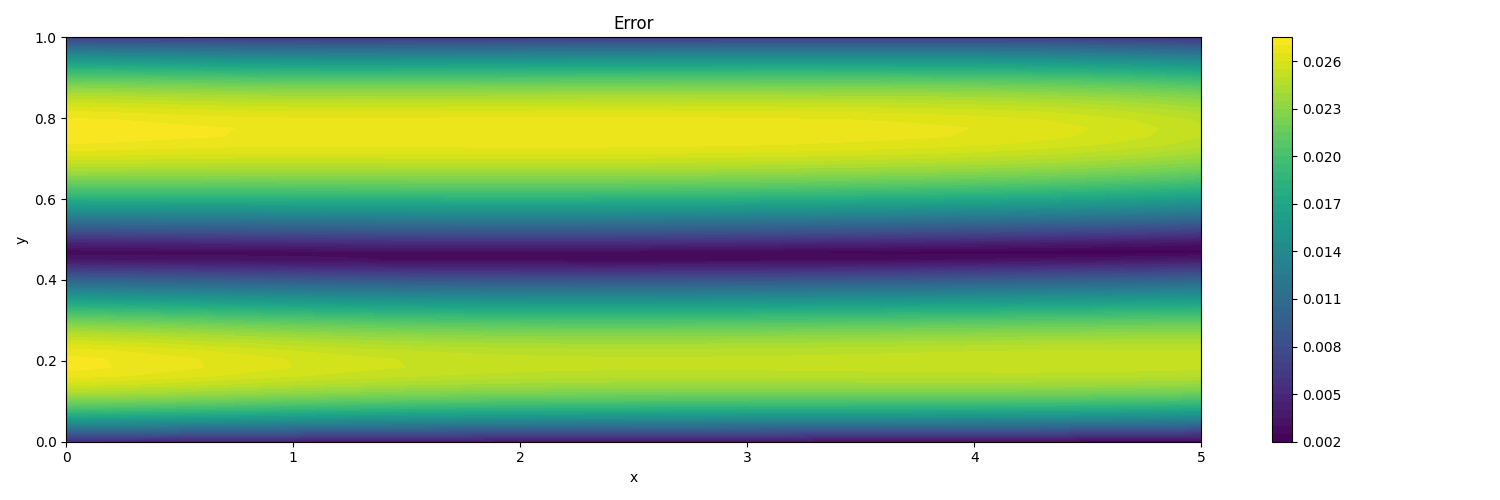
\includegraphics{data/couette_abu_error_best.png}
    \caption{Результат с минимальным показателем отклонения от точного решения в процессе обучения и
    кроссвалидации модели с функцией активации ABU отобраный в результате анализа функции потерь}
    \label{fig:couette_abu_best}
\end{figure}

Однако как было отмечено при кроссвалидации функции потерь, имеется неоднозначность между
функцией потерь для уравнений Навье-Стокса и потерями на границах области. Хоть и были
получены результаты с низким процентом отклонения от точного решения, где максимальное
отклонение составило $2.6\%$, среди кроссвалидируемых результатов были и следующие
качественные модели (табл. \ref{table:couette_abu_best_models})

\begin{table}[ht]
    \centering
    \caption{Качественные модели при разных коэффициентах}
    \begin{tabular}{ |c|c|c|c|c|c| } 
        \hline
        Номер модели & $\beta_0$ & $\beta_1$ & $\beta_2$ & $\beta_3$ & Отклонение, \% \\
        \hline
        $1$ & $1$ & $1$ & $1$ & $0$ & $1.125$ \\ 
        \hline
        $2$ & $1$ & $1$ & $1$ & $0$ & $1.800$ \\ 
        \hline
        $3$ & $1$ & $1$ & $1$ & $0$ & $2.600$ \\ 
        \hline
        $4$ & $1$ & $1$ & $0$ & $0$ & $2.880$ \\ 
        \hline
        $5$ & $1$ & $1$ & $0$ & $0$ & $2.250$ \\ 
        \hline
        $6$ & $0$ & $1$ & $1$ & $1$ & $4.500$ \\ 
        \hline
        $7$ & $0$ & $1$ & $1$ & $1$ & $2.700$ \\ 
        \hline
    \end{tabular}
    \label{table:couette_abu_best_models}
\end{table}

Как можно заметить, некоторые модели имеют одни и те же коэффициенты, но
разные результаты. Это связано с тем, что результат модели также 
зависит от начальной инициализации весов, которая каждый раз
генерируется случайным образом.

Исходя из таблицы \ref{table:couette_abu_best_models} лучшая модель
выдала результат (рис. \ref{fig:couette_abu_best_model}) с максимальным отклонением в $1.125\%$.

\begin{figure}[ht]
    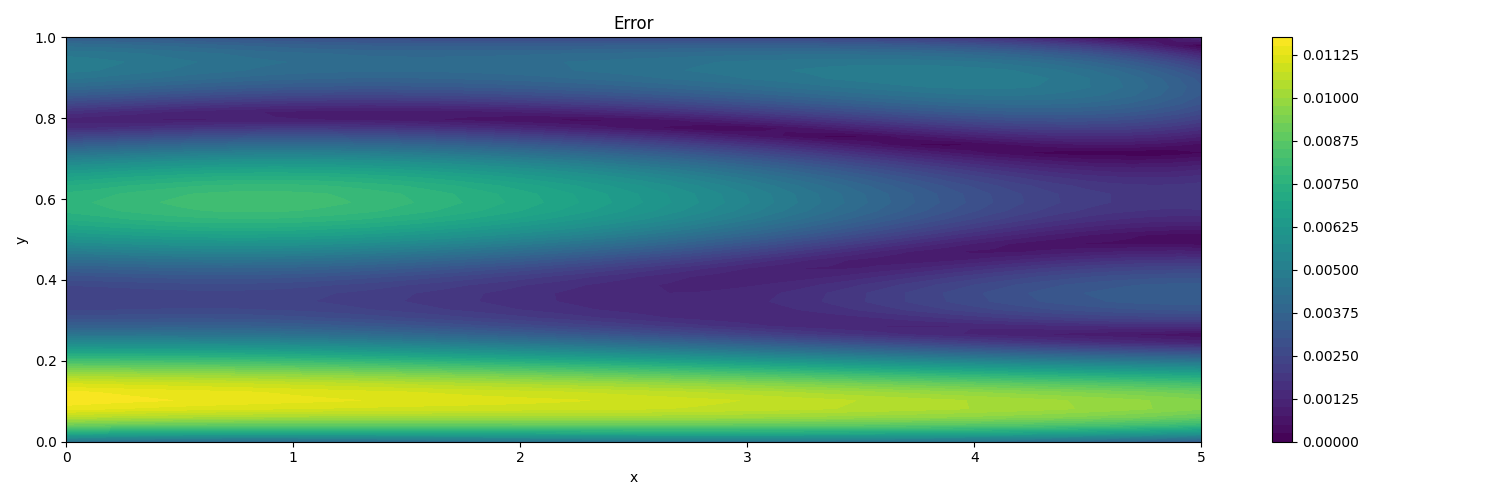
\includegraphics{data/couette_abu_error_best_model.png}
    \caption{Результат с минимальным показателем отклонения от точного решения в процессе обучения и
    кроссвалидации модели с функцией активации ABU отобраный в результате ручного анализа}
    \label{fig:couette_abu_best_model}
\end{figure}

Можно заметить, что оптимизатор и количество слоев совпало
с результатами кроссвалидации, в отличии от параметров
функции активации. Как упоминалось ранее, это связано с
малой выборкой параметров $\beta_i$, а также с присутствием
в выборке плохо обученных моделей. 

\chapter*{Заключение}
\addcontentsline{toc}{chapter}{Заключение}

В процессе анализа поведения физически-информированной нейронной сети были выявлены
закономерности и зависимости от гиперпараметров, на которые следует обращать внимание
при настройке модели для конкретной задачи.

Практическая значимость подхода заключается в уменьшении необходимости в большом объёме
экспериментальных данных, ускорении вычислений и возможности эффективного использования
современных вычислительных платформ (CPU, GPU, NPU). Это открывает перспективы для применения
PINN в таких сферах, как игровая и киноиндустрия, где требуется быстрое и реалистичное
моделирование жидкостей.

В работе проведён анализ влияния различных параметров нейронной сети (структуры, функций
активации, методов оптимизации) на качество решения. Особое внимание уделено выбору
функций активации, показано преимущество адаптивных и комбинированных функций (например,
ABU-PINN) для задач с различными физическими свойствами.

Результаты тестирования на задаче течения Куэтта с известным аналитическим решением подтвердили
способность PINN воспроизводить физически корректные распределения скоростей и давления,
а также выявили влияние архитектурных решений на точность модели.

Выбор правильного оптимизатора позволяет избегать нулевых решений, если это позволяет
функция активации. Количество точек внутри области и на ее границах, а если быть точным,
их отношение, влияет на то, какой из уравнений в постановке задачи будет отдан приоритет.
Конкретного соотношения нет, поэтому следует проводить кроссвалидацию как можно с большим
количеством вариантов. Функция активации в основном влияет на решение внутри области в
силу своей главной задачи --- внести нелинейность. 

Также были сравнены функции активации ABU и REAct, в результате которого были сделаны выводы,
что ABU пусть и медленнее, но намного точнее справляется со своей задачей.

Основные ограничения связаны с необходимостью подбора архитектуры сети под конкретную задачу
и возможной нестабильностью обучения при сложных физических условиях. Тем не менее, подход PINN
демонстрирует высокую гибкость и потенциал для дальнейшего развития.

Физически-информированные нейронные сети являются перспективным инструментом для моделирования
гидродинамических процессов, обеспечивая высокую точность и устойчивость решений при минимальных
требованиях к объёму экспериментальных данных. Дальнейшее развитие этой технологии связано с
оптимизацией архитектур, расширением области применения и интеграцией с другими методами машинного
обучения и численного моделирования.